\chapter{Mạng neural và Mạng neural tích chập (Convolutional Neural Networks CNN}

\section{Mạng neural (Neural Network)}

\subsection{Mạng neural ( Neural Network )}
	
	
	Theo khái niệm về sinh học, mạng neural là sự kết nối giữa các tế bào thần kinh neural lại với nhau. Trong lĩnh vực trí tuệ nhân tạo, mạng neural còn được gọi là Artificial Neural Network (ANN) - mạng neural nhân tạo, đây là mô hình xử lý dữ liệu, mô phỏng lại chức và cách hoạt động của hệ thống neural sinh học ở con người. Hình \ref{fig:neuron} minh họa cấu trúc của tế bào thần kinh neuron.
	
	\begin{figure}[h!]
		\centering
		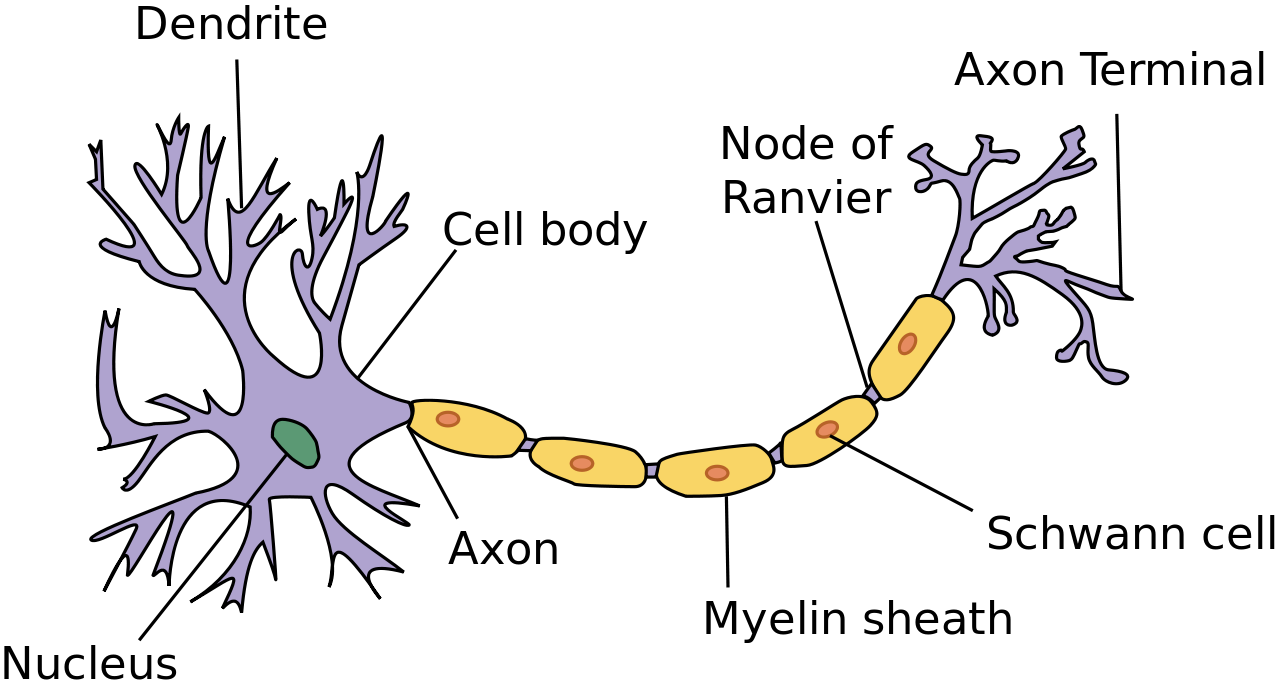
\includegraphics[scale=0.18]{charts/neuron.png}
		\caption{Tế bào thần kinh neuron sinh học \cite{img-neuron}}
		\label{fig:neuron}
	\end{figure}
	
	Mạng neural có gồm nhiều đơn vị kết nối, làm việc như một thể thống nhất thông qua việc trao đổi thông tin nhờ các liên kết.
	
	\subsection{Cấu trúc mạng neural}
	Như đã trình bày, các neuron trong một mạng làm việc như một thể thống nhất bằng việc trao đổi thông tin. Thực tế, đây là quá trình điều chỉnh các trọng số được truyền từ input ban đầu kết hợp với các hàm tính toán để có được các thông số trọng số phù hợp nhất. Quá trình này còn được gọi là quá trình học hay huấn luyện. Hình \ref{fig:NN} mô tả cấu trúc đơn giản nhất của một mạng neuron.
	\begin{figure}[h!]
		\centering
		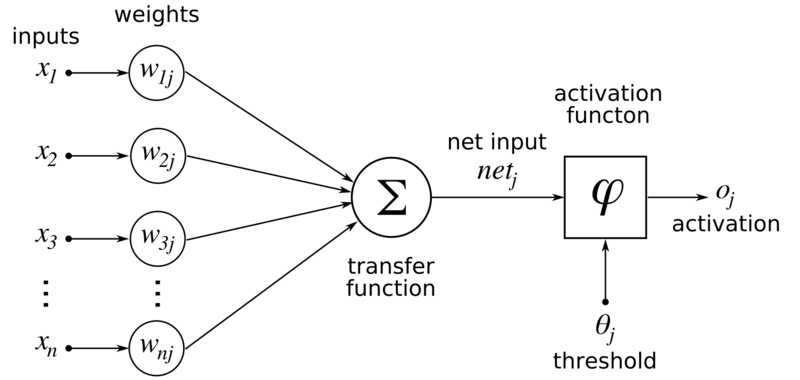
\includegraphics[scale=0.4]{charts/NN.png}
		\caption{Cấu trúc cơ bản mạng neuron\cite{img-perceptron}}
		\label{fig:NN}
	\end{figure}
	
	\textbf{Cấu trúc mạng neuron\i}
	
	\begin{itemize}
		\item \textbf{Tập các node:} bao gồm nhiều node, mỗi node là đơn vị nhỏ nhất giữ chức năng xử lý thông tin của mạng.
		\item \textbf{Các tầng:} Các node trên được xếp thành các tầng, các node chung một tầng không thể kết nối nhau. Trong đó tầng input và tầng output là 2 tầng thiết yếu. Tùy vào một số mạng cụ thể có thể có thêm một hay nhiêu tầng nằm ở giữa được gọi là tầng ẩn (hidden layer).
		\begin{itemize}
			\item \textbf{\textit{Tầng input - input layer: }}các nối ở tầng này nhận dữ liệu đầu vào và truyền tới các node ở các tầng kế tiếp, trong một số trường hợp còn có chức năng xử lý thông tin.
			\item \textbf{\textit{Tầng ẩn - hidden layer: }}một số mạng có thể có thêm tầng ẩn, số lượng tầng ẩn trong một mạng có thể nhiều hơn 1. Có chức năng nhận các giá trị từ từng input hoặc tầng ẩn trước nó, tính toán các giá trị và gửi đến các node ở các tầng ẩn hoặc tầng ouput tiếp theo đó tùy theo từng mạng cụ thể.
			\item \textbf{\textit{Tâng output - output layer: }}nhận giá trị từ tầng trước đó (tầng ẩn hoặc tầng input) để tính toán các giá trị ngõ ra.
		\end{itemize}
		\item \textbf{Các liên kết:} mỗi node trong một tầng truyền thông tin qua các node ở các tầng khác thông qua các liên kết. Các giá trị mà các liên kết này được gán sẽ được gọi là trọng số liên kết (weight). Giá trị trọng số được kết nối vào neuron j với neoron k là \(w_{kj}\).
		\item \textbf{Hàm truyền - transfer function: }dùng để tính tổng các tích input với trọng số liên kết của nó. \[ \sum input_j*w_{ij}\]
		
		\item \textbf{Activation function: }dùng để tính toán giá trị input sang giá trị ouput. Tùy vào mục địch và cụ thể từng loại mạng mà có nhiều loại activation function khác nhau.\\
		Trong các bài toán khác nhau, người có những loại hàm activation như sau.
		
		\begin{itemize}
			\item \textbf{\textit{Step function: }} 
			\[ 
			\left \{
  			\begin{tabular}{cc}
  				0 & x < 0\\
  				1 &  x > 0 
  			\end{tabular}
		\right.
		\]
		\pagebreak
		\begin{figure}[h!]
			\centering
			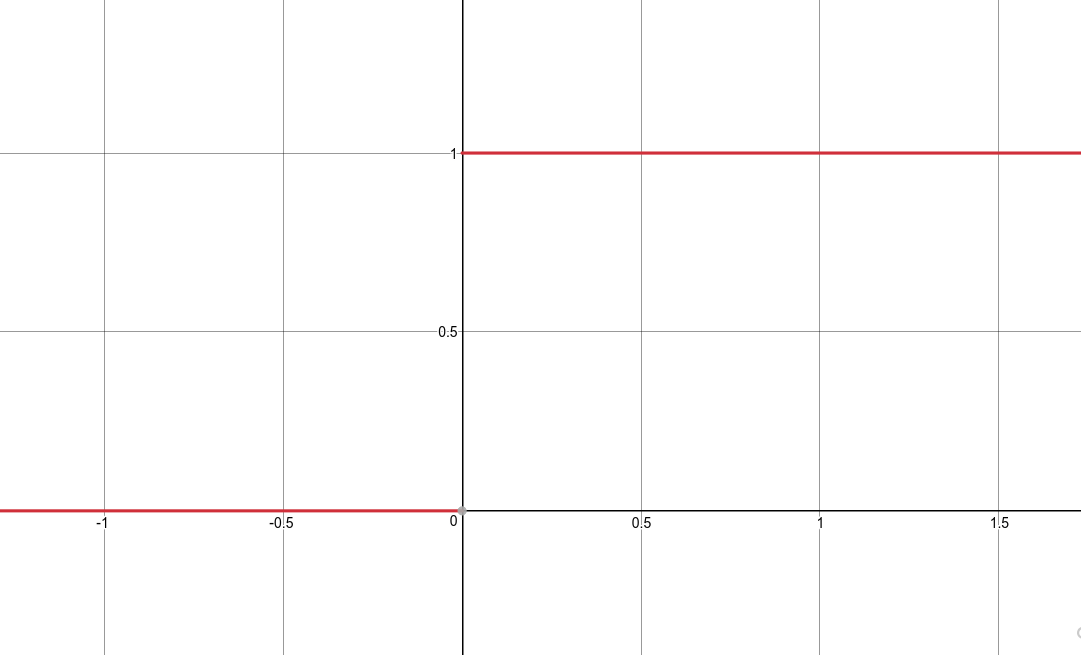
\includegraphics[scale=0.2]{charts/step_fun.png}
			\caption{Đồ thị hàm step}
			\label{fig:plot_step}
		\end{figure}
		
			\item \textbf{\textit{sigmoid function: }}
			\[A(x) =  \frac{1}{1 + e^{-x}}	\]
			\begin{figure}[h!]
				\centering
				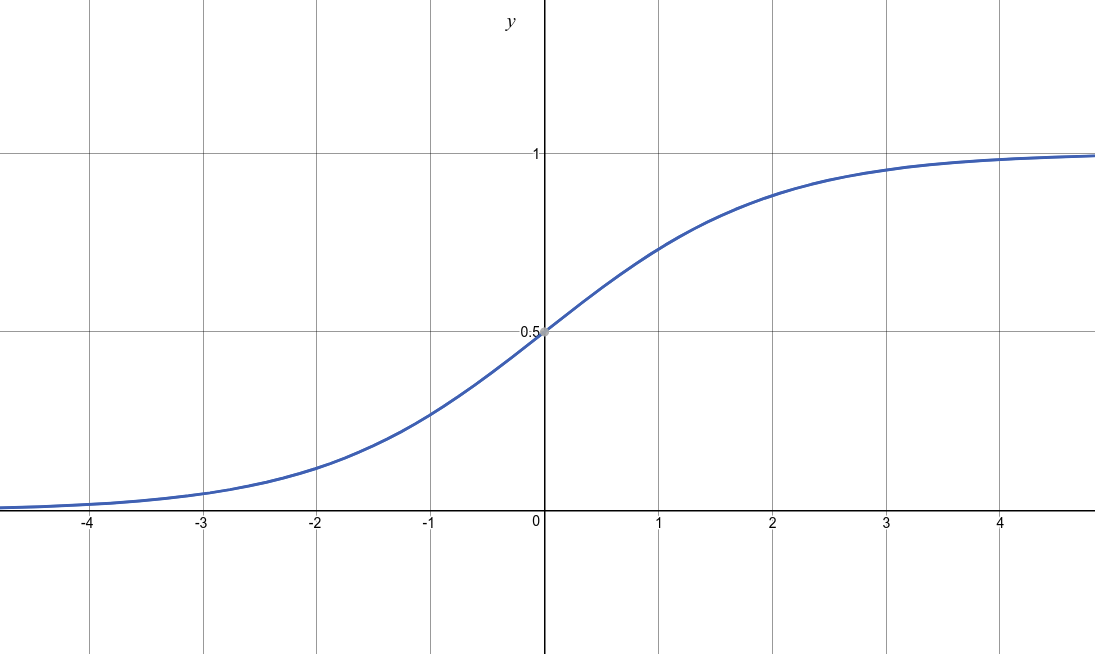
\includegraphics[scale=0.2]{charts/sigmoid_fun.png}
				\caption{Đồ thị hàm sigmoid}
				\label{fig:plot_sigmoid}
			\end{figure}
			
			\item \textbf{\textit{Tanh function:}}
			\[Tanh(x) = \frac{2}{1 + e^{-2x}} - 1 \]
			\begin{figure}[h!]
				\centering
				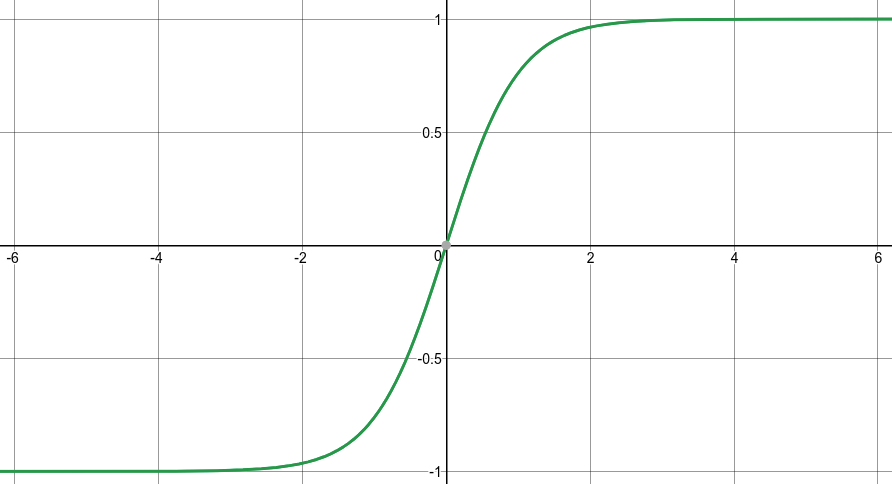
\includegraphics[scale=0.2]{charts/tanh_fun.png}
				\caption{Đồ thị hàm Tanh}
				\label{fig:plot_tanh}			
			\end{figure}
			
		\end{itemize}
		
	\end{itemize}
	
	\subsection{Mô hình Feedforward Neural Network}
	
		Thời điểm hiện nay, chúng ta có rất nhiều loại mô hình mạng neuron do sự khác nhau về sự kết hợp cũng như về mặt kiến trúc và thuật toán mà mạng đó áp dụng. Trong phần này, chúng ta sẽ tìm hiểu về mô hình mạng Feedforward Neural Network (FFNN), đây là kiến trúc mạng neuron được sử dụng phổ biến trong các bài toán dự báo. Mô hình gồm hai thành phần chính đó là kiến trúc feedforward - mạng truyền thẳng và giải thuật Backpropogation được áp dụng trong mạng.
		\subsubsection{Kiến trúc Feedforward}
			Đối với mạng feedfroward, cấu trúc gồm một tầng input, một tầng output và có thể có nhiều hơn một tầng ẩn nằm giữa hai tầng input và output. \\
			\begin{figure}[h!]
				\centering
				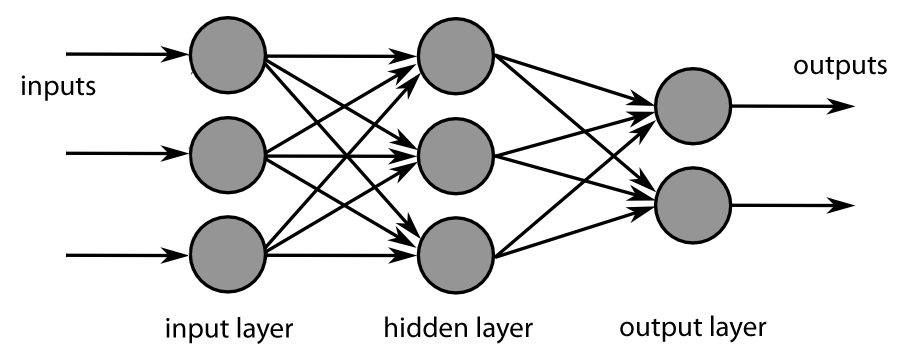
\includegraphics[scale=0.3]{charts/ffnn.png}
				\caption{Ví dụ kiến trúc mạng feeddorward \cite{ffnn-img}}
				\label{fig:ffnn}			
			\end{figure}\\
			Như hình \ref{fig:ffnn}, một mạng Feedorward, trong tầng input và ouput thì số lượng neuron tại mỗi hai tầng nãy sẽ là cố định tùy theo đặc tính của dữ liệu. Đối với tầng ẩn, số lượng tầng ẩn cũng như số lượng neuron trong mỗi tầng tùy thuộc vào cá nhân thiết kế.
			
		\subsubsection{Giải thuật Backpropogation}
		Ở nội dung này, chúng ta sẽ không đi sâu vào kỹ thuật xử lý các phép tính\cite{dl} đạo hàm mà chỉ trình bày giải thuật lan truyền ngược một cách đơn giản nhất.\par
		Các ký hiệu và hàm được dùng trong trình bày giải thuật:
		\begin{itemize}
			\item \(W_{ij}\): là trọng số nối node thứ i tới node j ở layer kế tiếp.
			\item \(I_{j}\): là đầu vào tại node thứ j.
			\item \(O_{j}\): là kết quả xuất tại node thứ j.
			\item \(\theta_{j}\): bias tại node j.
			\item \(l\): tốc độ học của mạng (learning rate).
			\item \(Err_{j}\): giá trị lỗi tại node thứ j.
			\item Activation function được dùng trong nội dung này là hàm Sigmoid như mục trên
		\end{itemize}
		
		\begin{figure}[h!]
			\centering
			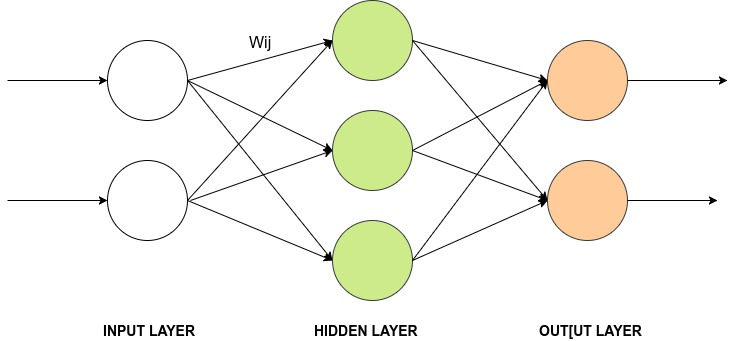
\includegraphics[scale=0.5]{charts/back.jpg}
			\caption{MLP}
			\label{fig:back}
		\end{figure}
		\pagebreak
		Nội dung thuật toán.\par
		\textbf{Input:}
		\begin{itemize}
			\item Mạng feed forward với n input, m node ở tầng ẩn, và p output.
			\item Hệ số học hay tốc độ học \(l\).
			\item Tập dữ hiệu huấn luyện \(D\).
			\item Sai số học \(\epsilon\).
		\end{itemize}
		\textbf{Output:} Vector các trọng số mới sau khi huấn luyện.
		
		\textbf{Nội dung thuật toán:}
		
		\begin{itemize}
			\item \textbf{Bước 1:} Khởi tạo ngẫu nhiên các giá trị trọng số  \(W_{ij}\).
			\item \textbf{Bước 2:} Tính toán các giá trị đầu vào \(I_{j}\) và đầu ra \(O_{j}\).
			\begin{itemize}
				\item Tại node i ở tầng input:
				\[I_{i} = x_{i}, O{i} = I_{i}\]
				\item Tại node j ở tầng khác:
				\[ I_{j} = \sum_{i} W_{ij}O_{i} + \theta_{j} \]
				\[O_{j} = \frac{1}{1 + e^{-I_{j}}}\]
			\end{itemize}
			\item \textbf{Bước 3:} Tính toán lỗi trung bình và đánh giá.
				\begin{itemize}
					\item Tại node thuộc tầng output:
					\[Err_{j} = O_{j}(1-O_{j})(T_{j} - O_{j})\]
					\item Tại node thuộc tầng ẩn:
					\[Err_{j} = O_{j}(1-O_{j})\sum_{k}Err_{k}W_{jk}\]
					Với \(Err_{k}, W_{jk}\) là giá trị lỗi tại node k ở tầng tiếp theo và giá trị trọng số của node j đến k.\\
					Thuật toán sẽ dừng lại khi \(Err_{k} \leq \epsilon\)
					
				\end{itemize}
			\item \textbf{Bước 4:} Cập nhật các trọng số và độ lệch
			\[W_{ij} = W_{ij} + (l)Err_{j}O_{i}\]
			\[\theta_{j} = \theta_{j} + (l)Err_{j}\]
			
			Thuật toán sẽ tiếp tục lặp lại bước 2 cho đến khi thỏa điều kiện dừng và cho ra các tập trọng số và độ lệch tốt nhất.
		\end{itemize}
		
		
		
		
			
			

\section{Mạng neural tích chập (Convolutional neural network)}

\subsection{Giới thiệu mạng neural tích chập}
	Trong vài năm trở lại đây, chúng ta thấy được sự nở rộ của các hệ thống thông minh từ các công ty công nghệ lớn trên thế giới. Các chức năng nhận dạng, phân loại hay dự đoán được áp dụng rộng rãi vào các lĩnh vực thương mại, vận tải..v..v.\par
	Mô hình Deep learning được sử dụng phổ biến và phát triển giúp các hệ thống thông minh có độ chính xác cao ngày nay chính là Convolutional Neural Networks(CNN) - mạng neuron tích chập. Trong các nội dung tới, chúng ta sẽ tìm hiểu các khái niệm, kiến trúc, cũng như ứng dụng của CNN trong lĩnh vực phân loại ảnh.

\subsection{Mô hình mạng neural tích chập}
	\subsubsection{Input và output}
		Phân loại ảnh là công đoạn chuyển hóa từ một đầu là một hình ảnh và kết quả là một nhãn ứng với hình ảnh đó hoặc là các xác suất mà hệ thống dự đoán dựa trên đặc điểm của ảnh. Với con người, công việc nhận diện này được hình thành từ khi mới sinh ra, chúng ta có thể đưa ra kết quả của một hình ảnh bất kỳ mà không chút khó khăn. Nhưng máy tính thì không đơn giản như vậy, đầu vào và kết quả phải được đưa về dạng kỹ thuật số mà máy có thể hiểu được.\par
		Khi một máy tính nhận vào một ảnh, nó sẽ thấy một mảng các giá trị pixel tùy thuộc vào kích thước và độ phân giải của ảnh\cite{overview}. Ví dụ, một ảnh màu có kích thước 224 x 224 pixel thì máy tính sẽ thấy hình ảnh này dưới dạng một mảng có kích thước 224 x 224 x 3, giá trị 3 do thuộc tính ảnh màu(RGB) mà có được, giá trị này sẽ là 1 nếu đây là ảnh trắng đen.\par
		Đối với ouput, đây là một mảng các giá trị xác suất, mảng giá trị này cũng tùy thuộc vào số lượng nhãn(lớp) cần dự đoán. Ví dụ, (0.90 cho xe ô tô, 0.1 cho xe tải).
	\subsubsection{Convolutional layer}
		Tầng đầu tiên của một mạng CNN luôn luôn là tầng tích chập (convolutional layer)\cite{conv}. Như đã biết đầu vào (input) là một mảng các giá trị pixel. Trong trường hợp cụ thể để dễ hình dung ta chọn input là mảng các giá trị pixel có kích thước 32 x 32 x 3 với 32 x 32 là chiều dài và chiều rộng của tấm hình và 3 là giá trị RGB khi là ảnh màu. Đối với input trên có nghĩa là sẽ có một ma trận có kích thước 32 x 32 pixel mỗi pixel sẽ chứa 3 giá trị mà mỗi giá trị đó lần lượt biểu diễn cho giá trị của 3 màu sắc trên máy tính là đỏ(RED), lục(GREEN) và làm(BLUE). \par
		Tạm thời bỏ qua giá trị RGB để đi vào cách hoạt động của tầng tích chập này. Cách đơn giản để giải thích cách hoạt động của tầng tích chập là tưởng tượng sẽ có một khuôn sẽ trượt từ phía trên bên trái cho đến hết tấm ảnh\cite{arch}. Với kích thước ảnh là 32 x 32 như trên, chọn kích thước ô trượt ví dụ là 5 x 5. Ô trượt có kích thước 5 x 5 sẽ trượt lần lượt qua cả input ảnh, ô trượt này được gọi là kernel hay filter(bộ lọc). Bộ lọc là một mảng các giá trị trọng số. Một điểm ghi chú là chiều sâu của bộ lọc sẽ bằng với chiều sâu của ảnh, với input 32 x 32 x 3 thì bộ lọc cũng sẽ có 5 x 5 x 3. Hình \ref{fig:conv_layer1} và \ref{fig:conv_layer2} minh họa cách kernel trượt trên input.
		%\pagebreak
		\begin{figure}[h!]
			\centering
			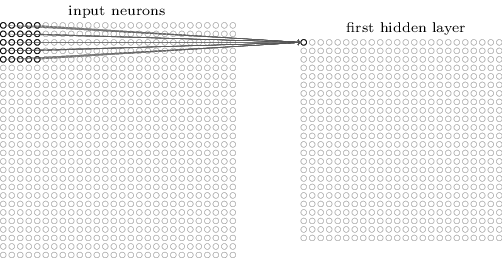
\includegraphics[scale=0.8]{charts/conv_layer1.png}
			\caption{Convolutional layer \cite{conv-layer}}
			\label{fig:conv_layer1}
		\end{figure}
		
		\begin{figure}[h!]
			\centering
			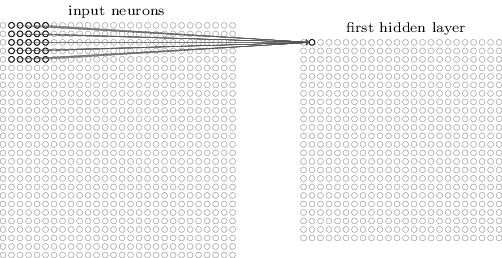
\includegraphics[scale=0.8]{charts/conv_layer2.png}
			\caption{Convolutional layer \cite{conv-layer}}
			\label{fig:conv_layer2}
		\end{figure}
		
		Bây giờ ta sẽ đi vào việc mà tầng tích chập thực sự làm với những phép tính. Như đã trình bày rằng mỗi bộ lọc sẽ là một mảng các giá trị pixel, công dụng của mảng giá trị này nhằm mục đích phát hiện các đặc tính của mỗi vùng input mà filter trượt qua. Các đặc tính ở đây có thể là đường thẳng, đường cong, màu đơn giản. Ví dụ ta có một filter có kích thước là 7 x 7 x 3 dùng để phát hiện một dạng đường cong như hình \ref{fig:filter}.
		
		\begin{figure}[h!]
			\centering
			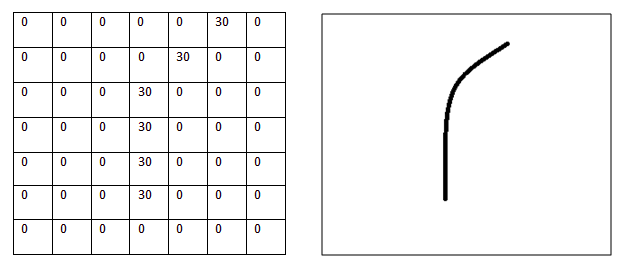
\includegraphics[scale=0.5]{charts/filter.png}
			\caption{Mảng các giá trị của bộ lọc \cite{conv-layer}}
			\label{fig:filter}
		\end{figure}
		
		Khi bộ lọc trên trượt đến vùng được đánh dấu vàng có dạng đường cong giống với bộ lọc như hình \ref{fig:mouse}. Lúc đó phép toán   tích châpj sẽ được thực hiện như hình \ref{fig:conv_1} với ma trận bên trái chính là giá trị pixel của vùng được đánh dấu trên ảnh mà bộ lọc trượt tới, ma trận bên phải chính là bộ lọc được sử dụng hiện tại.
		
		\begin{figure}[h!]
			\centering
			
\includegraphics[scale=0.5]{charts/mouse.png}
			\caption{ảnh đầu vào \cite{img-input}}
			\label{fig:mouse}
		\end{figure}
		\pagebreak
		
		\begin{figure}[h!]
			\centering
			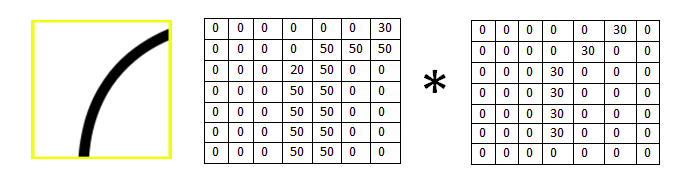
\includegraphics[scale=0.5]{charts/conv_1.png}
			\caption{phép toán tích chập \cite{img-input}}
			\label{fig:conv_1}
		\end{figure}
		
		Kết quả của phép tính trên sẽ có kết quả như sau:
		\[(50*30)+(50*30)+(50*30)+(20*30)+(50*30) = 6600 \]\\
	
		Đây là một con số rất lớn, thông thường nếu bộ lọc trượt tới một vùng mà vùng đó có hình dạng tương tự như bộ lọc thì kết quả khi thực hiện phép tính là một con số rất lớn. Ngược lại, kết quả sẽ ra rất nhỏ hoặc bằng 0. Ví dụ là hình ảnh \ref{fig:conv_2} kết quả sẽ là 0 khi thực hiện phép tính
		\begin{figure}[h!]
			\centering
			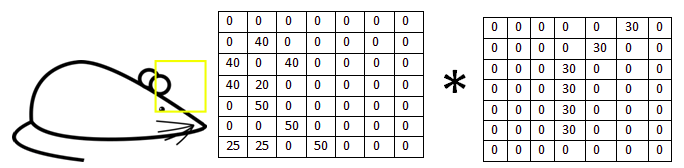
\includegraphics[scale=0.5]{charts/conv_2.png}
			\caption{phép toán tích chập \cite{img-input}}
			\label{fig:conv_2}
		\end{figure}
		
		Trên đây là mô tả đơn giản về tầng tích chập, trên thực tế, chúng ta có thể có nhiều bộ lọc để phát hiện các khuôn mẫu, hình dạng khác nhau trong ảnh đầu vào. Kết quả xuất của tầng tích chập thứ nhất còn được gọi là bản đồ đặc tính (feature map) và có thể có nhiều feature map cho một input sau khi hoàn thành tầng tích chập. Như \ref{fig:feature_map} biểu diễn một input kích thước như hình sau khi qua tầng tích chập và sử dụng tập các bộ lọc 5 x 5 cho ra tập 3 feature map mà mỗi cái nhận diện được một khuôn dạng khác nhau xuất hiện trong input.
		%\pagebreak
		\begin{figure}[h!]
			\centering
			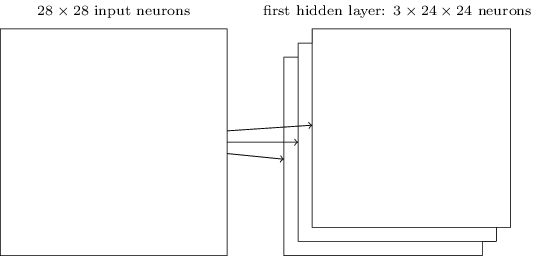
\includegraphics[scale=0.5]{charts/feature_map.png}
			\caption{kết quả tầng tích chập \cite{img-input}}
			\label{fig:feature_map}
		\end{figure}
	
	\subsubsection{Pooling Layer}		
		Sau khi qua một hoặc vài tầng tích chập, CNN sẽ chứa các tầng tổng hợp (Pooling Layer) ngay sau đó. Ở đây, tầng tổng hợp sẽ đơn giản hóa thông tin được lấy từ đầu ra từ tầng tích chập trước đó. Có nhiều kiểu tổng hợp khác nhau đối với tầng này, nhưng max-pooling là phép tổng hợp phổ biến được sử dụng. Hình \ref{fig:max-pooling} biểu diển một ví dụ phép max-pooling với một bộ lọc có kích thước là 2 x 2. Giá trị lớn nhất trong mỗi vùng được trượt qua sẽ được chọn làm kết quả xuất ra.
		
		\begin{figure}[h!]
			\centering
			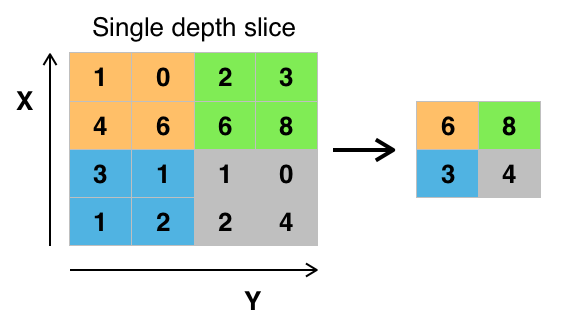
\includegraphics[scale=0.7]{charts/max_pooling.png}
			\caption{max-pooling 2 x 2 \cite{img-pool}}
			\label{fig:max-pooling}
		\end{figure}
		\pagebreak
		
		Công dụng của phép pooling này giúp giảm đi kích thước của tập miêu tả đặc trưng từ đó cũng làm cho số lượng tham số và tính toán giảm theo. Và do chúng ta có thể có nhiều feature map từ tầng tích chập nên phép tổng hợp cũng sẽ được áp dụng độc lập cho mỗi feature map. Nếu có 3 feature map thì sẽ có 3 phép tổng hợp trong trường hợp này là max-pooling.
		
		\begin{figure}[h!]
			\centering
			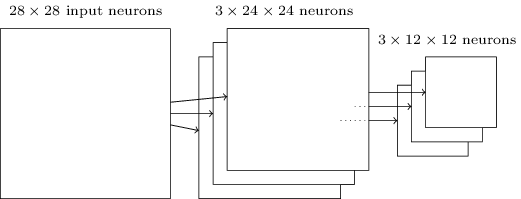
\includegraphics[scale=0.5]{charts/pooling_ex.png}
			\caption{Ví dụ tầng tổng hợp \cite{conv-layer}}
			\label{fig:pooling_ex}
		\end{figure}
		
	
	\subsubsection{Fully Connected Layer}
		Sau khi thông tin input đã qua các tầng tích chập và tổng hợp, các giá trị dữ liệu sẽ đi đến tầng fully connected để xuất ra kết quả. Kết quả tại tầng fully connected là một vector có kích thước bằng với số lớp(nhãn) mà bài toán cần dự đoán. Như bài toán phân loại ảnh giao thông ùn tắt và thông thoáng thì lúc này số nhãn cần dự đoán và kích thước vector tại tầng này sẽ bằng 2. Giá trị của các phần tử trong vector sẽ là giá trị xác suất của mỗi nhãn mà mạng dự đoán, [ 0.8, 0.2 ] sẽ biểu diễn 80\% ảnh này thuộc lớp 1 và 20\% ảnh thuộc lớp thứ 2. Về cơ bản, cách kết nối ở tầng này giống như cách kết nối neuron giữa các tầng với nhau ở mạng neuron ở mục trước. Khi đó, tất cả neuron ở tầng pooling sẽ kết nối với từng neuron trong tầng cuối.
	
\subsection{Kiến trúc mạng GoogLeNet)}
	
	\subsubsection{Ý tưởng}
	Đây là kiến trúc mạng tích chập với 22 tầng. GoogLeNet còn là quán quân của ILSVRC 2014 \cite{1}. Mạng googLeNet có cấu trúc mạng nằm trong mạng, có 9 tầng mà mỗi tầng là một inception module. Theo tài liệu cho biết, việc áp dụng inception module giúp làm giảm đáng kể số lượng tham số tính toán giúp giải quyết vấn đề về tài nguyên. \ref{fig:googlenet} minh họa cho cấu trúc của mạng googLeNet.
	
		
	\begin{figure}[h!]
			\centering
			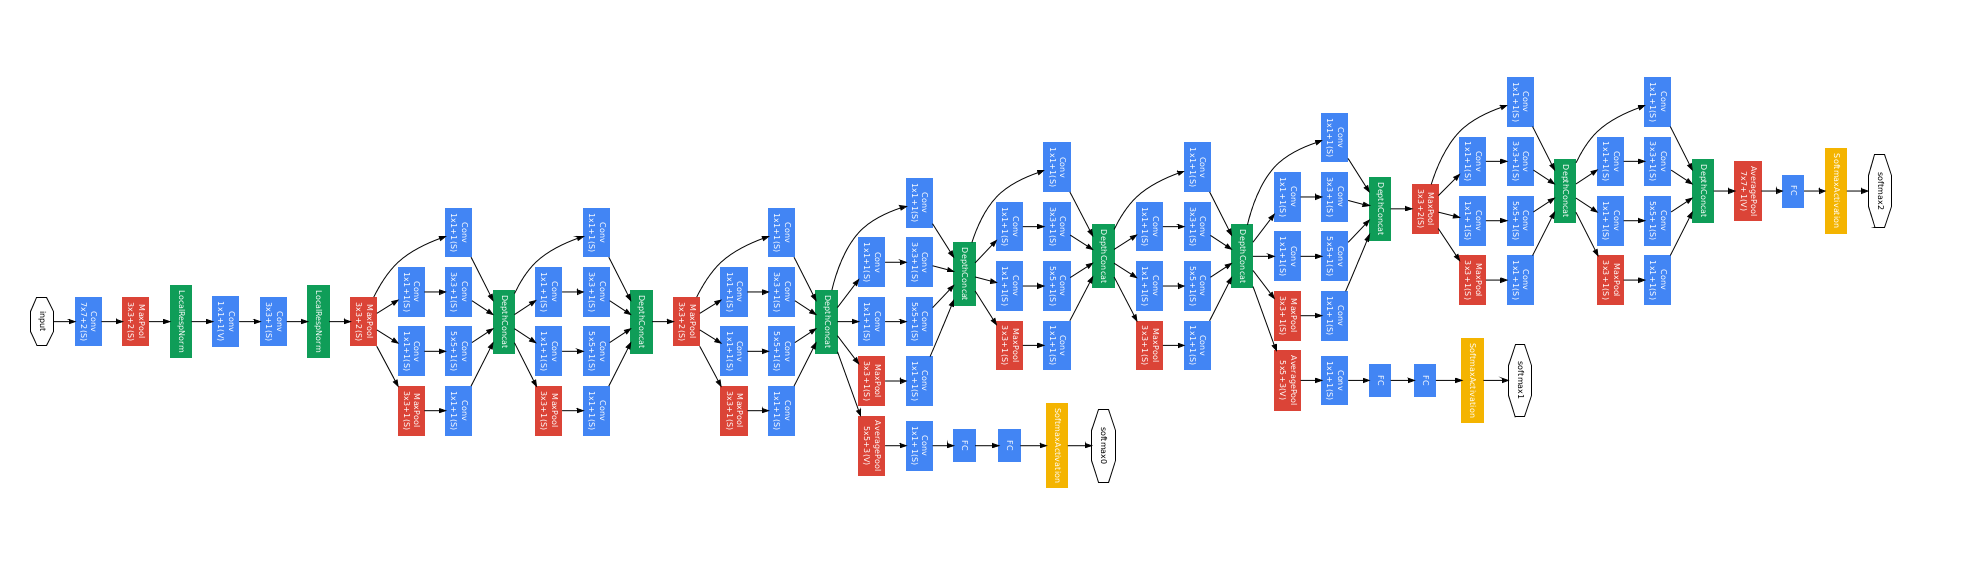
\includegraphics[scale=0.7]{charts/googlenet.png}
			\caption{GoogLeNet \cite{1}}
			\label{fig:googlenet}
		\end{figure}
		
	
	\subsubsection{Inception module}
	Với minh họa kiến trúc của mạng googLeNet, ta sẽ thấy các layer là một khối mạng nhỏ nằm bên trong. Đây là các inception module. Đối với các mạng tích chập thông thường, khi một tập dữ liệu bắt đầu đi vào một tầng thì sẽ chỉ có hai sự lựa chọn đó chính là tầng tích chập hoặc tầng tổng hợp, nhưng với googLeNet sẽ có tập input sẽ đi vào một lớp module tại đó sẽ các phương thức tích chập và pooling sẽ đươc tính toán một cách song song và độc lập với nhau \cite{1}.
	
	\begin{figure}[h!]
			\centering
			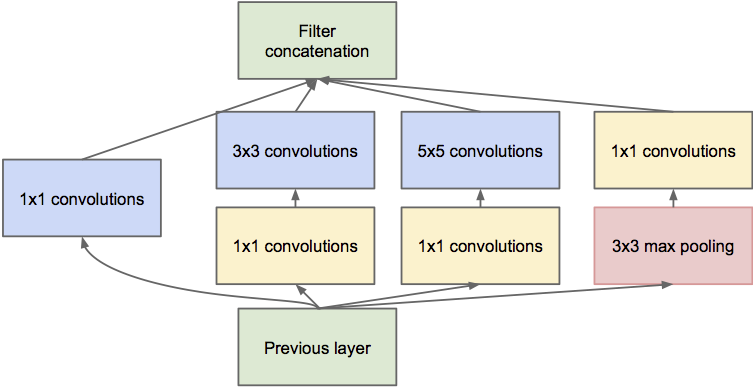
\includegraphics[scale=1.5]{charts/inception.png}
			\caption{inception module \cite{1}}
			\label{fig:inception}
	\end{figure}

	\begin{figure}[h!]
			\centering
			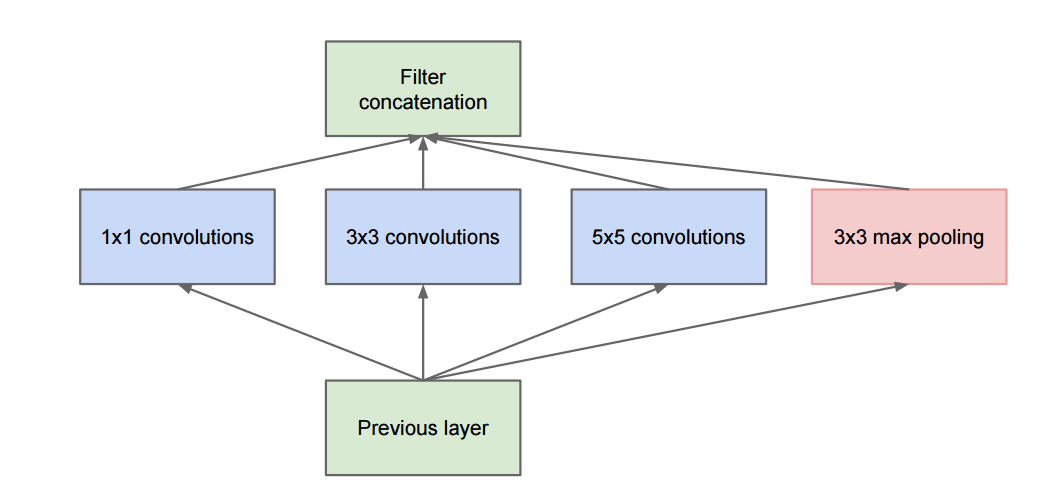
\includegraphics[scale=0.3]{charts/inception_nai.png}
			\caption{naive inception module \cite{1}}
			\label{fig:nai_inception}
	\end{figure}
		
	
	
	Hình \ref{fig:inception} miêu tả cấu trúc của một module trong mạng. Trong khi đó \ref{fig:nai_inception} là một ý tưởng ban đầu mà tác giả đã nghĩ tới. Ở \ref{fig:inception} chúng ta thấy trước khi thực hiện các phép tích chập với các filter 3 x 3 và 5 x 5, input đều được xử lý qua phép tích chập với filter 1 x 1. Các bộ lọc 1 x 1 có tác dụng làm giảm đi chiều của các input\cite{2}, điều này giúp cho khối lượng tham số phải tính toán ở phép toán tích chập với bộ lọc 3 x 3 và 5 x 5 sẽ được giảm đi một cách đáng kể.

		
	
	
	
	
	
